\documentclass[%
 reprint,
 amsmath,amssymb,
 aps,
]{revtex4-1}

\usepackage{graphicx}% Include figure files
\usepackage{dcolumn}% Align table columns on decimal point
\usepackage{bm}% bold math
\usepackage[dvipdfm,colorlinks=true,linkcolor=blue,filecolor=blue, urlcolor=blue]{hyperref}
\usepackage{braket}
\usepackage{caption} % captionsetup[figure]用
\usepackage{threeparttable} % Table のキャプションを変更
\usepackage{breqn} %dmath用：数式の自動折り返し
\numberwithin{equation}{section}% (p.37)

% \sloppy はすべての文章を「緩め」に設定し、オーバーフローや不均一な単語間隔を許すため、厳密な組版が求められる論文では推奨されません。
\tolerance=1000
\emergencystretch=1em
\hyphenpenalty=3000
\exhyphenpenalty=3000
\flushbottom
\usepackage[final]{microtype}
\usepackage{ragged2e} % 均等割付けのために追加

% Figsにも均等割付けをする(2023/12/24)
\captionsetup{
    format=plain,
    justification=justified,
    singlelinecheck=false}

\captionsetup[figure]{justification=raggedright,
labelfont={bf},name={Fig.},labelsep=period} %Fig.の注釈を左揃えするためrangedrightを用いる
\captionsetup[table]{labelfont={bf},name={Table.},labelsep=period}



\begin{document}

\title{Bridging Quantum Mechanics and General Relativity: \\ A First-Principles Approach to Anomalous Magnetic Moments and Geodetic Precession}

\author{Satoshi Hanamura}
\email{hana.tensor@gmail.com}
\date{January 25, 2025}
%\date{\today}


\begin{abstract}
Bridging quantum mechanics and general relativity remains one of the fundamental challenges in modern physics. While these theories have been extensively validated in their respective domains, their reconciliation at microscopic scales continues to be a subject of intense study. This work establishes a direct algebraic connection between the anomalous magnetic moments of leptons and their Zitterbewegung velocities, unifying quantum mechanical phenomena with both special and general relativistic principles. Our initial special relativistic calculations predicted electron Zitterbewegung velocities of $0.040472c$. However, by incorporating general relativistic effects through geodetic precession and utilizing the calculated muon critical radius of $3.43 \times 10^{-25}$ meters, we refined this prediction to $0.040374c$. We further determine critical radii of $5.71 \times 10^{-24}$ meters for tau leptons, where their Zitterbewegung motion becomes unsustainable. This result naturally explains both the tau-to-muon and muon-to-electron decay processes while reinforcing the stability of electron motion. By analyzing the interplay of Lorentz contraction and geodetic precession, we propose a hypothesis for a mass-dependent transition point between classical and quantum gravitational regimes, implying that general relativistic corrections may play a role in influencing quantum mechanical phenomena at microscopic scales.
\end{abstract}

\maketitle


\section{Introduction}

The quantum mechanical behavior of elementary particles, particularly the phenomenon known as \textit{Zitterbewegung} (trembling motion), represents a fundamental challenge in modern physics. Originally predicted by Schrödinger through the Dirac equation~\cite{Schrodinger1930}, Zitterbewegung has been traditionally interpreted as a light-speed oscillatory motion arising from matter-antimatter interactions through virtual particle collisions, presenting an unresolved paradox in quantum mechanics~\cite{Barut1981}. The present work, based on the 0-Sphere model~\cite{Hanamura2018} and its fundamental constituents called \textit{kernels} (Appendix \ref{sec:WhatIsThe0Sphere}), proposes an interpretation where Zitterbewegung occurs at subluminal velocity, specifically around 4\% of light speed for electrons. This reinterpretation, supported by recent theoretical advances~\cite{Hanamura2023}, suggests that the anomalous magnetic moment of electrons is directly connected to these microscopic oscillations between the kernels, providing a geometric framework for both Zitterbewegung and \textit{geodetic precession}.

By unifying special relativistic effects, such as Lorentz contraction, with general relativistic effects, such as geodetic precession, this work offers a comprehensive theoretical framework for understanding the interplay between gravity and quantum mechanics. By applying this methodology, we discovered that as particle radius decreases, the geodetic precession from general relativity increases, effectively counteracting the Lorentz contraction effects arising from the magnetic moment in special relativity. Through the calculation of the muon's critical radius, we were able to apply geodetic precession to Zitterbewegung, revealing a subtle but significant difference between purely special relativistic predictions ($v_{e,\text{SR}} = 0.040472c$) and those incorporating general relativistic effects ($v_{e,\text{SR+GR}} = 0.040374c$).

Our analysis reveals how general relativistic corrections fundamentally alter our understanding of particle behavior. This study identifies specific critical radii where quantum effects intersect with relativistic phenomena: $3.43 \times 10^{-25}$ meters for muons and $5.71 \times 10^{-24}$ meters for tau leptons. These radii mark crucial transitions in particle stability, offering a geometric explanation for the observed decay patterns in the lepton family.

Similarly, when we applied the electron's anomalous magnetic moment and mass to the critical radius where muon Zitterbewegung velocity reaches zero, we found that electrons remain stable at this radius, experiencing minimal geodetic precession effects at muon critical radii. These mathematical relationships connecting anomalous magnetic moments with geodetic precession suggest the potential for applying general relativity principles to quantum mechanical systems. This leads to a novel hypothesis: tau particles and muons reach the end of their lifetime when their Zitterbewegung velocity becomes zero. Furthermore, this framework provides insights into why lepton generations decay specifically to electrons, offering a geometric perspective on generational hierarchy in the lepton family.

The remainder of this paper is organized as follows. Section~\ref{sec:TheoreticalFramework} presents the theoretical framework, including the electron's structure in our model, quantum mechanical foundations, and detailed velocity analyses incorporating both special and general relativistic corrections. Section~\ref{sec:Discussion} discusses the implications of our findings for particle decay processes and their relationship with Standard Model predictions. Finally, Section~\ref{sec:Conclusion} concludes with a summary of our key findings and their significance for understanding the interface between quantum mechanics and general relativity.


\clearpage


\section{Theoretical Framework}
\label{sec:TheoreticalFramework}


\subsection{Revisiting Zitterbewegung: A Transition from Relativistic to Subluminal Oscillation}
\label{sec:RevisitingZitterbewegung}

Recent advancements in the author's research propose that Zitterbewegung occurs at a subluminal velocity, approximately $0.04c$ for electrons. This reinterpretation transforms Zitterbewegung from an abstract quantum effect into a measurable physical velocity.

The Zitterbewegung phenomenon has traditionally been understood as rapid oscillatory motion occurring at the speed of light due to interference between the \textit{positive energy solutions} and \textit{negative energy solutions} of the Dirac equation. In conventional physics, Zitterbewegung has been interpreted as an oscillatory term arising from the interaction between positive and negative wavefunctions in the Dirac equation, attributed to electron-positron interactions. However, as discussed in the previous section, our research reinterprets the positive and negative wavefunctions of the Dirac equation as representing two kernels. These kernels are composed of thermal potential energy (TPE), and the model has been reinterpreted to describe the physical transfer of TPE through radiation between discrete positions from one Kernel to another.
Consequently, in the 0-Sphere model, Zitterbewegung does not require electron-positron pairs to occur. Instead, it manifests as a sinusoidal radiation gradient within a single electron. For the geometric calculation process by which the 0-Sphere model generates sine waves through thermal radiation, refer to Appendix \ref{sec:ThermalEnergyGradient}.

In Zitterbewegung, positive and negative energy solutions evolve independently in time as long as no external forces are applied. This means that a \textit{wave packet} constructed solely of positive energy solutions will not contain negative energy solutions even as time passes. However, it has been traditionally interpreted that both positive and negative energy solutions are generally necessary to localize waves in a finite region. The single-electron model with two kernels applied in the 0-Sphere model interprets these kernels as positive and negative energy solutions, while the photon gas surrounding the two kernels is expressed in the kinetic energy term.

As a result, this theory is consistent with the conventional assertion that both positive and negative energy solutions are necessary to localize a Dirac particle wave packet to approximately the length of its Compton wavelength divided by $2\pi$. In the 0-Sphere model, this wave packet is not interpreted as a mixture of plane waves as traditionally applied in the Schrödinger equation. This reinterpretation stems from viewing the single electron as a composite structure consisting of physical kernels and tangible photon gas. Additionally, since the two kernels exist at spatially discrete positions on the order of the Compton wavelength, this theory holds potential as a theory that can avoid ultraviolet divergence.

The mechanism for avoiding ultraviolet divergence can be understood through the oscillatory motion of the photon sphere performing Zitterbewegung vibrations between two spatially separated kernels at the Compton wavelength scale. During this motion, the photon sphere undergoes simple harmonic acceleration and deceleration. When we consider the interaction where photons are emitted from or absorbed into the photon sphere during each finite cycle of acceleration and deceleration, the ultraviolet divergent interactions cannot occur infinitely many times. This is because infinite interactions would require infinite energy.

Building on the author's 0-Sphere model, this framework connects Zitterbewegung to the anomalous magnetic moment of particles, incorporating general relativistic corrections through geodetic precession. Key predictions include the critical radius for muons, the corrections to electron velocities, and the implications for particle decay processes. These insights pave the way for experimental verification and offer a unified perspective that integrates quantum mechanics with relativistic principles.


\subsection{Reconstructing Electron Structure:\\ The Dual-Kernel Approach}
\label{sec:ReconstructingElectronStructure}

In the 0-Sphere electron model, an electron's structure is assumed as follows. First, consider there are tiny thermal sources in the center. These thermal spots, named kernels in author's previous papers already submitted, can transfer energy between them via radiation. These two kernels are geometrically analogous to the two points represented by the 0-Sphere (See Appendix \ref{sec:WhatIsThe0Sphere}). Next, consider a real photon gas that surrounds the two kernels. The photon sphere gas confines and maintains electromagnetic interaction with the kernels, which constitute the bare electron.

The concept of the photon gas has not changed since mentioned on paper \cite{Hanamura2018, Hanamura2023}. The photons surrounding the two thermal sources exchanging energy with each other are real photons. Because the photon is connected to the thermal spot by the electromagnetic force, this photon does not emit energy to the external system and cannot be observed. In this paper, one electron is regarded as a closed system in thermodynamics, and this paper is not expanded to the interaction with other electrons. From this viewpoint, this real photon gas may have been called a virtual photon. However, the virtual photons used in the past are particles that are temporarily generated during an interaction, and the meaning of the virtual photons in this paper is very different in that they do not satisfy the energy conservation law.

While it is generally accepted that positive and negative energy solutions represent electrons and positrons respectively, this model presents a different interpretation. Traditionally, in the Dirac representation, the Dirac spinor exhibits a mixing between its upper and lower two components, which are typically separated through appropriate unitary transformations. In contrast, this study interprets the positive and negative solutions derived from the Dirac equation as representing two kernels existing within a single electron~\cite{Hanamura2020}. This interpretation eliminates the need to separate the rest energy from the four-component wave function $\psi$ obtained from the Dirac equation.

Unlike conventional quantum mechanics, which allows for temporary violations of energy conservation through quantum fluctuations, the 0-Sphere model demonstrates that a single electron maintains perfect energy conservation throughout all temporal phases, with no energy fluctuations. This strict adherence to the conservation law persists regardless of the phase in the oscillation cycle, challenging the traditional acceptance of quantum uncertainty in energy conservation. The 0-Sphere model provides a deeper mechanism for electron stability: rather than static existence, the electron maintains its stability through a dynamic equilibrium of continuous energy exchange between its constituent kernels. Unlike tau leptons and muons, electrons never reach a critical radius where Zitterbewegung oscillations become unsustainable, instead maintaining perpetual oscillatory motion through this energy exchange process.



\begin{figure*}[t!]
    \centering 
    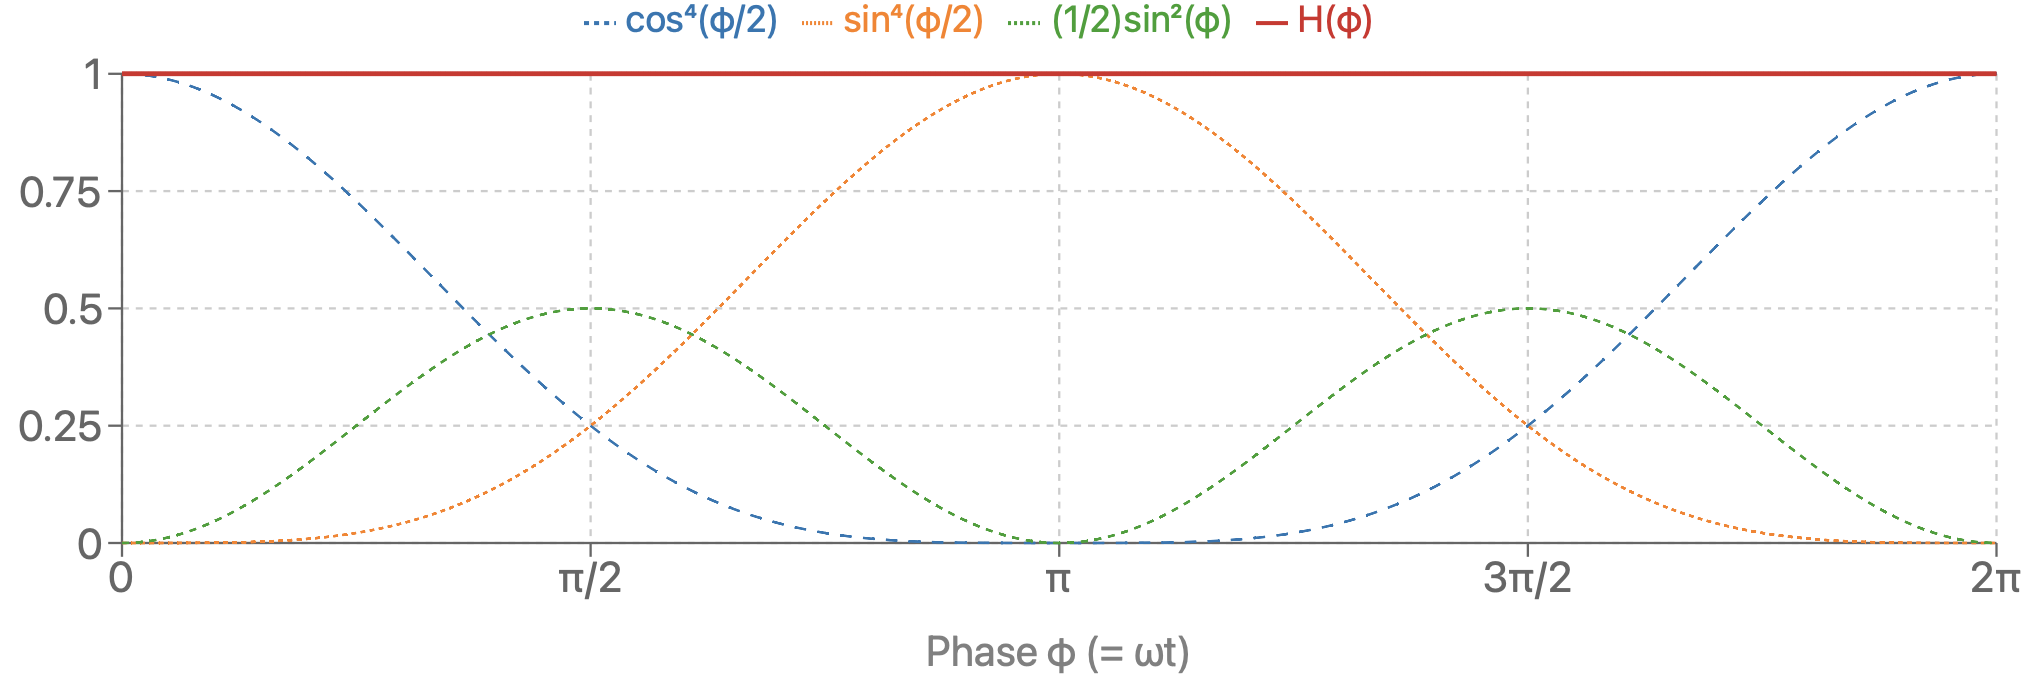
\includegraphics[width=\textwidth]{f-TotalHamiltonian.png}
    \caption{\justifying Visualization of energy conservation in the 0-Sphere model. The graph shows the time evolution of various energy components: the complementary oscillations of the thermal potential energy (TPE) terms $\cos^4(\phi/2)$ and $\sin^4(\phi/2)$, representing kernels $A$ and $B$ respectively, and the double-frequency oscillation of the kinetic energy term $(1/2)\sin^2(\phi)$ of the photon sphere. At $\phi=0$, Kernel $A$ possesses all rest energy as TPE, while at $\phi=\pi$, Kernel $B$ contains all TPE, and at $\phi=2\pi$ the cycle completes with Kernel $A$ again containing all TPE. The total energy remains constant at a value of 1 throughout the complete cycle. Kernels $A$ and $B$ represent TPEs that are discretely separated in space, and these points are geometrically represented as a 0-sphere. For details on the 0-sphere: $S^0$ and $n$-sphere: $S^n$, see Appendix.~\ref{sec:WhatIsThe0Sphere}. In the energy transfer process $e^-_{\mathrm{thermalA}} \rightarrow \gamma^*_{\mathrm{K.E.}} \rightarrow e^-_{\mathrm{thermalB}}$, the blue dashed line represents $e^-_{\mathrm{thermalA}}$, the yellow dashed line $e^-_{\mathrm{thermalB}}$, and the green dashed line the photon sphere's kinetic energy $\gamma^*_{\mathrm{K.E.}}$.}
    \label{f-TotalHamiltonian}
\end{figure*}


\subsection{Dynamic Stability Mechanism of Electrons:\\ Energy Exchange Between Kernels}
\label{sec:DynamicStabilityMechanism}

This study offers an interpretation of lepton lifetimes through the lens of geodetic precession. By examining how particles respond to this general relativistic effect, we can explore the relationship between particle mass and stability, particularly in the context of tau lepton and muon decay processes. When these particles reach their respective critical radii, as will be demonstrated in subsequent sections, their Zitterbewegung velocities approach zero, suggesting a potential mechanism for generational transitions in the lepton family:

\begin{equation}
\tau^- \rightarrow \mu^- + \bar{\nu}_\mu + \nu_\tau,
\end{equation}

\begin{equation}
\mu^- \rightarrow e^- + \bar{\nu}_e + \nu_\mu.
\label{eq:MuonDecay}
\end{equation}

This raises a fundamental question: Why doesn't the electron decay? Conventional physics posits that the electron has an infinite lifetime, but the 0-Sphere model offers a more nuanced interpretation. While electrons don't decay in the same manner as tau leptons or muons, they undergo a continuous process of renewal through their Zitterbewegung oscillations. The stability mechanism can be understood by examining the electron's fundamental structure. In the 0-Sphere electron model, the electron's structure includes two kernels exchanging energy through a photon sphere. The thermal potential energy (TPE) of Kernel $A$ transforms into kinetic energy via the photon sphere, which then transfers to Kernel $B$. This process can be represented as:

\begin{equation}
e^-_{\mathrm{kernelA}} \rightarrow \gamma^*_{\mathrm{K.E.}} \rightarrow e^-_{\mathrm{kernelB}}.
\label{eq:electron_transfer}
\end{equation}
Here, $\gamma^*_{\mathrm{K.E.}}$ represents the photon sphere, which converts the rest energy of Kernel $A$ containing TPE into kinetic energy, and is subsequently reabsorbed into Kernel $B$. This process is formalized by Eq. (\ref{eq:total_hamiltonian}), which will be discussed later (see Fig. \ref{f-TotalHamiltonian} for visualization). This formulation suggests that while individual kernels may have finite lifetimes, the electron as a whole maintains stability through continuous energy exchange. Unlike tau leptons and muons, electrons never reach a critical radius where Zitterbewegung oscillations become unsustainable. Instead, they maintain their oscillatory motion indefinitely through this perpetual exchange of energy between kernels.

The thermal energy terms $e^-_{\mathrm{kernelA}}$ and $e^-_{\mathrm{kernelB}}$ in Eq. (\ref{eq:electron_transfer}) correspond to the $\cos^4(\omega t/2)$ and $\sin^4(\omega t/2)$ terms of TPE, respectively, where $E_0$ is the rest energy of a single electron, as described by:
\begin{equation}
E_{0} = E_{0} \left( \cos^{4} \left( \frac{\omega t}{2} \right) + \sin^{4} \left( \frac{\omega t}{2} \right) + \frac{1}{2} \sin^{2} (\omega t) \right).
\label{eq:total_hamiltonian}
\end{equation}

Equation (\ref{eq:total_hamiltonian}) demonstrates that at time phase $\omega t=0$, Kernel $A$ possesses all rest energy as TPE, while at time phase $\omega t=\pi$, Kernel $B$ holds all rest energy as TPE. The process represented in Eq. (\ref{eq:electron_transfer}) does not occur in discrete phases; rather, as $e^-_{\mathrm{kernelA}}$ begins to decay, $e^-_{\mathrm{kernelB}}$ simultaneously begins to accumulate TPE. For a detailed visualization of this TPE phase transition over time, refer to Fig. \ref{f-TotalHamiltonian}. As shown in the figure, the TPE from $e^-_{\mathrm{kernelA}}$ is not directly transferred to $e^-_{\mathrm{kernelB}}$ in its entirety.

At any given time $t$, a portion of the energy exists as kinetic energy in $\gamma^*_{\mathrm{K.E.}}$, as demonstrated by Eq. (\ref{eq:total_hamiltonian}). This geometric interpretation provides new insight into the single-electron structure, where kinetic and potential energies have traditionally been considered inseparable. Moreover, this model suggests that during these quantum oscillations, energy is strictly conserved at all phases, challenging the conventional understanding of energy uncertainty in quantum states. Equation (\ref{eq:total_hamiltonian}) thus offers a novel perspective on the quantum state of a single electron, where energy conservation is maintained even during microscopic oscillations.

This geometric interpretation not only preserves energy conservation but also provides insight into the fundamental nature of the kernels themselves. In the 0-Sphere model, Kernel $A$ and Kernel $B$ correspond to positive energy solutions and negative energy solutions, respectively. However, their roles are not fixed, as they continuously exchange positions through the process of radiation and absorption in time phase. Rather than definitively assigning Kernel $A$ and Kernel $B$ to positive and negative energy solutions, it is more appropriate to interpret the radiation-absorption correspondence itself as representing the positive and negative energy solutions. Within this framework, the oscillation of the photon sphere $\gamma^*_{\mathrm{K.E.}}$ manifests as the Zitterbewegung phenomenon, providing a geometric foundation for this quantum mechanical effect. A distinct feature of the 0-Sphere model, revealed through the rigorous structural analysis of Eq.~(\ref{eq:total_hamiltonian}), is that Zitterbewegung can geometrically occur within a single electron.



\subsection{Comparative Velocity Analysis of Leptons: Electron and Muon Dynamics}
\label{sec:ComparativeVelocityAnalysis}

Prior to delving into the detailed analysis, it is important to note that this research is grounded in the premise that anomalous magnetic moments arise from Lorentz contraction effects, specifically those induced by the sublight-speed microscopic oscillations of electrons. This perspective offers a framework for interpreting quantum corrections traditionally attributed to virtual particle interactions.
For readers who may be unfamiliar with this approach, a significant aspect of this work is the examination of the Thomas precession from a geometric perspective. Rather than viewing spin as a predetermined quantum property with entangled states representing superpositions, we explore how spin states can emerge from the harmonic oscillation of the electron, with up and down states periodically alternating with the temporal evolution of the oscillation cycle~\cite{Hanamura2023}.

\begin{figure}[t!]
    \centering 
    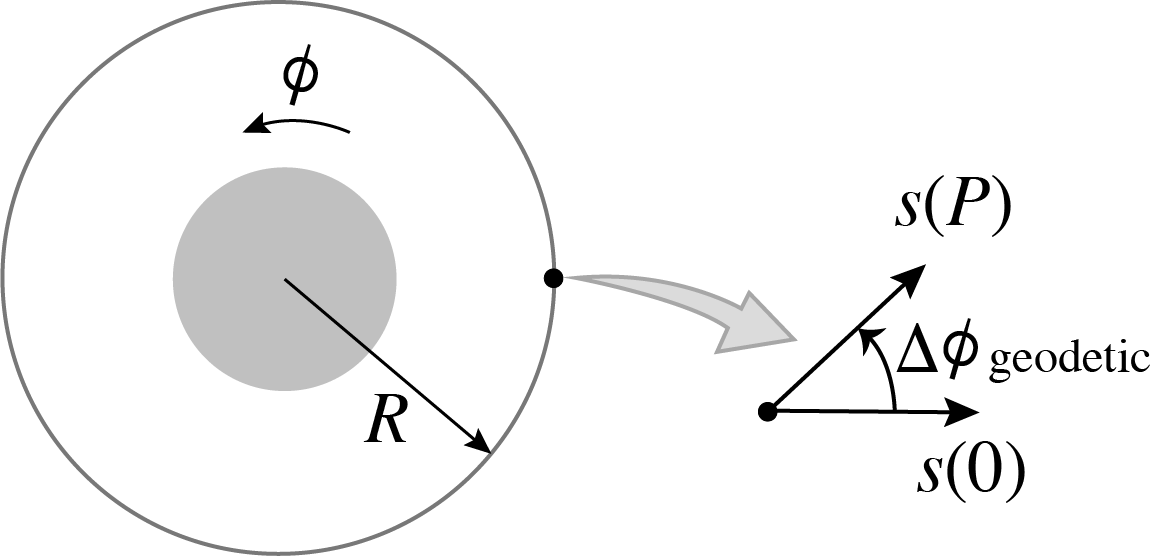
\includegraphics[scale=0.21]{geodetic.png}
    \caption{``Geodetic precession. This is a schematic view of the equatorial plane of a $\textit{nonrotating}$ spherical body. A gyroscope orbits in a circle of Schwarzschild coordinate radius $R$. At the start of one orbit at $t$ = 0, its spin is oriented in the radial direction. At the completion of one orbit, its spin has been rotated by an angle $\Delta \phi_{\mathrm{geodetic}}$ in the direction of orbital motion in a time $P = 2 \pi / \Omega$.'' See \cite{Hartle} for details.}
    \label{f_Geodetic}
\end{figure}

In this section, we review the equations connecting electron's anomalous magnetic moment with Lorentz contraction. The subsequent Results section will introduce corrections based on geodetic precession (see Fig.~\ref{f_Geodetic}), a concept from general relativity theory. The analysis investigates the Zitterbewegung velocity of electrons and muons based on their anomalous magnetic moment data. The anomalous magnetic moment, $a_\ell$, quantifies the deviation of the lepton's gyromagnetic ratio, $g_\ell$, from the classical Dirac value of 2~\cite{Schwinger1948}. This deviation arises due to quantum corrections, including contributions from virtual particles in quantum field theory. It is expressed mathematically as:

\begin{equation}
a_\ell = \frac{g_\ell - 2}{2},
\end{equation}
where $g_\ell$ represents the gyromagnetic ratio of the lepton. 

Traditionally, $a_\ell$ has been understood as an independent quantum mechanical quantity, with no direct connection to phenomena like Zitterbewegung. In this work, we examine a possible relationship that connects $a_\ell$ to the lepton's oscillatory motion. Specifically, we explore how Zitterbewegung, a rapid oscillatory motion predicted by the Dirac equation, might contribute to the quantum corrections that give rise to $a_\ell$. The electron's anomalous magnetic moment has served as a fundamental testing ground for quantum electrodynamics (QED). Through perturbative calculations up to order $\alpha^5$, QED predicts a theoretical value of~\cite{Aoyama2012,Aoyama2015,Nio2015}:

\begin{equation}
    a^{\text{theory}}_{\text{e}} = 0.001\,159\,652\,181\,643(764).
\end{equation}

However, our approach diverges from standard theoretical frameworks. Instead of relying on QED predictions, we utilize direct experimental measurements to explore the relationship between quantum mechanics and general relativity. The current experimental values for electrons and muons are~\cite{Fan2023, Bennett2006}:

\begin{equation}
   a^{\text{exp}}_{\text{e}} = 0.001\,159\,652\,180\,59\,(13),
   \label{eq:electron_moment}
\end{equation}

\begin{equation}
   a^{\text{exp}}_{\mu} = 0.001\,165\,920\,62\,(41).
   \label{eq:muon_moment}
\end{equation}
These experimental values provide the foundation for our analysis, offering a direct connection between measurable quantum phenomena and relativistic effects without relying on perturbative quantum field theory calculations~\cite{Hanneke2008}.

The analysis begins by considering the Lorentz contraction effects in the laboratory frame. Let $L_0$ denote the length in a coordinate system moving with the particle and $L$ represent the observed length from the laboratory system. The relationship follows the standard Lorentz contraction formula:

\begin{equation}
   L = L_0\sqrt{1 - \frac{v^2}{c^2}}.
   \label{eq:lorentz}
\end{equation}
To account for the oscillatory nature of particle motion, the analysis incorporates Root Mean Square (RMS) considerations for the anomalous magnetic moment. The factor $1/\sqrt{2}$ in our formulation specifically accounts for the time-averaging of the Zitterbewegung velocity. Without this factor, the equations would yield the instantaneous maximum velocity of the oscillation rather than the RMS average velocity. Including this factor in our analysis yields:

\begin{equation}
\frac{L}{L_0} = \frac{1}{1 + \frac{1}{\sqrt{2}}a^{\text{exp}}}.
\label{eq:length_ratio}
\end{equation}
This RMS averaging is particularly relevant for experimental considerations, as measuring the instantaneous velocity of Zitterbewegung would be technically more challenging than measuring its average velocity over one oscillation period.

Combining Eqs. (\ref{eq:lorentz}) and (\ref{eq:length_ratio}), the relationship becomes:

\begin{equation}
   \sqrt{1 - \frac{v^2}{c^2}} = \frac{1}{1 + \frac{1}{\sqrt{2}}a^{\text{exp}}}.
   \label{eq:combined}
\end{equation}
For the electron case, substituting the experimental value from Eq. (\ref{eq:electron_moment}) leads to:

\begin{equation}
   \beta^2_e = (\frac{v_e}{c})^2 = 0.00163798087,
   \label{eq:beta_electron}
\end{equation}

\begin{equation}
   v_{\text{electron}} = 0.04047197635 \times c.
   \label{eq:velocity_electron}
\end{equation}
The above results have already been calculated in paper~\cite{Hanamura2023}. In the next subsection, we will calculate the previously undetermined Zitterbewegung velocity of the muon.


For muons, substituting $a^{\text{exp}}_{\mu}$ from Eq. (\ref{eq:muon_moment}) provides a detailed calculation sequence:

\begin{equation}
   \begin{split}
       1 - \beta^2_{\mu} &= \frac{1}{(1 + \frac{1}{\sqrt{2}}a^{\text{exp}}_{\mu})^2} \\
       &= \frac{1}{(1 + \frac{1}{\sqrt{2}} \cdot 0.00116592062)^2} \\
       &= \frac{1}{(1 + 0.000824424)^2} \\
       &= \frac{1}{1.001650} \\
       &= 0.998351724.
   \label{eq:beta_muon_detailed}
   \end{split}
\end{equation}
Therefore:

\begin{equation}
   \begin{split}
       \beta^2_{\mu} &= 1 - 0.998351724 \\
       &= 0.001648276,
   \label{eq:beta_muon_squared}
   \end{split}
\end{equation}

\begin{equation}
   \begin{split}
       \beta_{\mu} &= \sqrt{0.001648276} \\
       &= 0.0405989, 
   \label{eq:beta_muon_final}
   \end{split}
\end{equation}

\begin{equation}
   v_{\text{electron}} = 0.0405989 \times c.
   \label{eq:velocity_muon}
\end{equation}
The calculated velocities demonstrate consistency between electrons and muons, differing only in the fourth decimal place despite their significant mass difference.




\section{Discussion}
\label{sec:Discussion}


\subsection{Relativistic Dynamics: Merging Special and General Relativity in Particle Behavior}
\label{sec:RelativisticDynamicsMerging}

Suppose at the start of an orbit the observer orients the gyro in a direction in the equatorial plane (say in the direction of a distant star). General relativity predicts that on completion of an orbit, the gyro will generally point in a different direction making an angle $\Delta \phi_{\mathrm{geodetic}}$ with the starting one. This change in direction is called geodetic precession~\cite{Everitt2011} and it's illustrated schematically in Fig. \ref{f_Geodetic}. 

It is important to note that electron spin has traditionally not been interpreted as a rotating body like a gyroscope. This interpretation stems from two fundamental considerations: first, a point particle cannot possess angular acceleration, and second, if conceived as a finite-radius sphere, it would violate the universal speed limit as parts of the rigid body would need to rotate faster than the speed of light. However, the 0-Sphere model, as demonstrated in the author's work~\cite{Hanamura2023}, introduces a crucial feature where particles can possess angular acceleration through Zitterbewegung-induced energy oscillations. Namely, electron spin has been modeled as an energy exchange through TPE oscillation. Through a reinterpretation of Thomas precession, it was mathematically proven that even linear acceleration can possess angular velocity. The author also demonstrated that if electron Zitterbewegung oscillates at approximately 4\% of the speed of light, the photon sphere of Compton wavelength order would not exceed the speed of light even at its equatorial plane~\cite{Hanamura2025-1}.

The spin comes back after one orbit rotated by an angle,
\begin{equation}
\Delta \phi_{\mathrm{geodetic}} = 2 \pi \left[ 1 - \left( 1 - \frac{3M}{R} \right)^{1/2} \right] \mathrm{(per \ orbit)},
\label{eq:Geodetic}
\end{equation}
in the direction of motion, as illustrated in Fig. \ref{f_Geodetic}. While another general relativistic effect known as the Lense-Thirring precession~\cite{LenseThirring1918} also exists, it is significantly smaller than the geodetic precession and therefore can be neglected in our analysis. 

In this study, we apply geodetic precession to the modified picture of electron spin, where TPE undergoes reciprocating motion in a straight line, rather than directly applying it to a rotating rigid body gyroscope. This systematic application of geodetic precession to the quantum mechanical behavior of electrons provides insights into potential connections between general relativity and quantum mechanics~\cite{Penrose1996}, contributing to the ongoing discussion in the field.



\subsection{Critical Radius: Derivations and Implications for Particle Stability}
\label{sec:CriticalRadiusDerivations}

The comparative analysis reveals that the geodetic precession effect exhibits a dramatic difference between electrons and muons, with the muon's precession being approximately two orders of magnitude larger than the electron's. This significant difference directly reflects the mass dependence of geodetic precession in general relativity, as the muon is about 206.77 times more massive than the electron.

At significantly larger radii ($r > 10^{-21}$ m), both particles exhibit remarkably stable velocities, with electrons maintaining $0.040472c$ and muons $0.040581c$, showing a minimal difference of about $0.27\%$. This near-constancy in velocities suggests that at these scales, the basic velocity is primarily determined by the anomalous magnetic moment, with geodetic effects being negligibly small for both particles.

Through precise mathematical analysis, we can now derive the exact critical radius where the Lorentz contraction ratio becomes unity. Starting with the condition where $L/L_0 = 1$:

\begin{equation}
   \frac{1}{1 + \frac{1}{\sqrt{2}}a^{\text{exp}}_{\mu} - \Delta\phi_g} = 1.
\label{eq:lorentz_ratio_start_corrected}
\end{equation}
Since $L/L_0 = 1$, this implies:
\begin{equation}
   1 + \frac{1}{\sqrt{2}}a^{\text{exp}}_{\mu} - \Delta\phi_g = 1,
\label{eq:basis_equation}
\end{equation}
where $\Delta\phi_g = \frac{\Delta \phi_{\text{geodetic}}}{2\pi} = 1 - \sqrt{1 - \frac{3m_{\mu}}{r_{\mu}}}$.

\noindent Substituting this expression and the known values:
\begin{equation}
\begin{aligned}
1 + & \frac{1}{\sqrt{2}}(0.00116592062) - \\
& \biggl(1 - \sqrt{1 - \frac{3 \times 1.883531627 \times 10^{-28}}{r_{\mu}}}\biggr) = 1
\end{aligned}
\label{eq:full_equation_corrected}
\end{equation}
Let $\frac{1}{\sqrt{2}}(0.00116592062) = 0.000824424$. Then:
\begin{equation}
   1 + 0.000824424 - 1 + \sqrt{1 - \frac{5.650594881 \times 10^{-28}}{r_{\mu}}} = 1
\label{eq:simplified_equation_corrected}
\end{equation}
Simplifying:
\begin{equation}
   0.000824424 + \sqrt{1 - \frac{5.650594881 \times 10^{-28}}{r_{\mu}}} = 1
\label{eq:further_simplified}
\end{equation}
Therefore:
\begin{equation}
   \sqrt{1 - \frac{5.650594881 \times 10^{-28}}{r_{\mu}}} = 0.999175576
\label{eq:sqrt_equation_corrected}
\end{equation}
Squaring both sides:
\begin{equation}
   1 - \frac{5.650594881 \times 10^{-28}}{r_{\mu}} = 0.998352115
\label{eq:squared_equation_corrected}
\end{equation}
Solving for $r_{\mu}$:
\begin{equation}
   \begin{split}
       -\frac{5.650594881 \times 10^{-28}}{r_{\mu}} &= -0.001647885\\
       r_{\mu} &= \frac{5.650594881 \times 10^{-28}}{0.001647885}\\
       &= 3.429069305573 \times 10^{-25}\\
       &\approx 3.43 \times 10^{-25} \text{ meters}.
   \end{split}
\label{eq:final_radius_corrected}
\end{equation}




\begin{figure*}[t!]
\centering
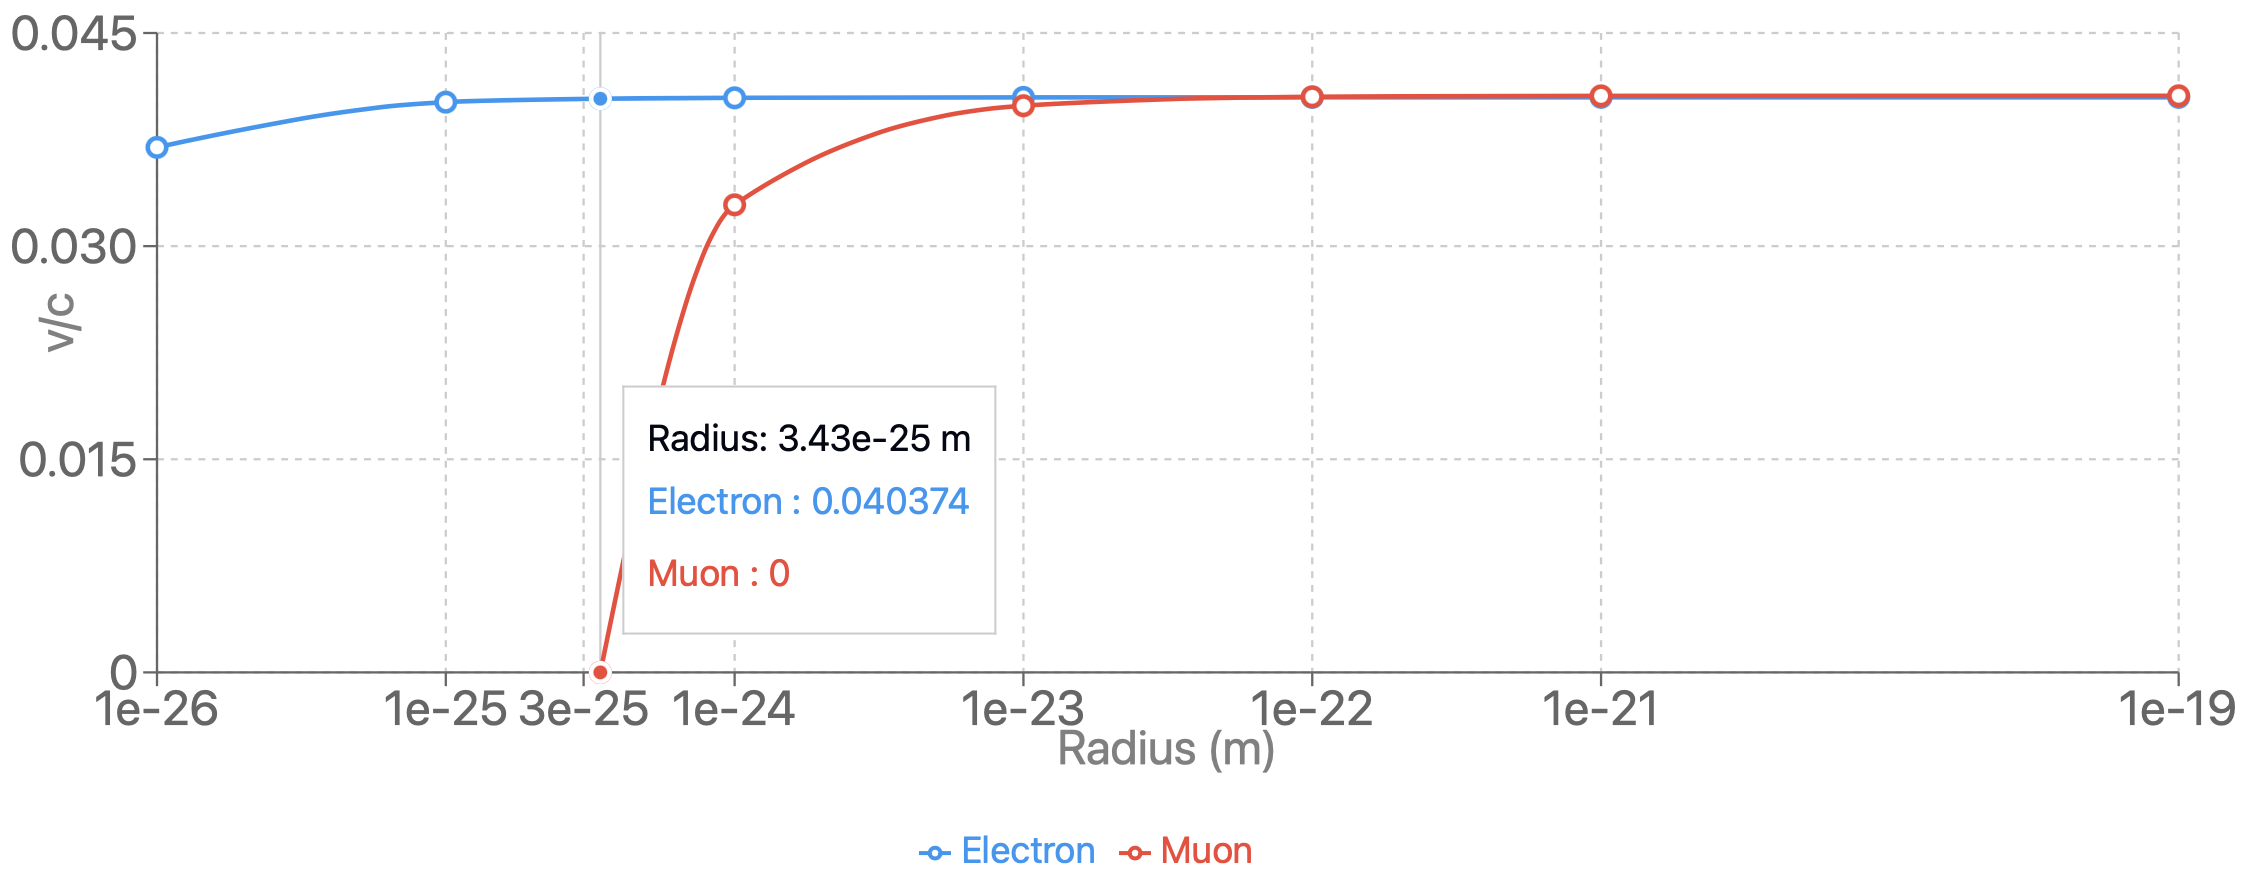
\includegraphics[width=\textwidth]{f-VelocityPlot.png}
\caption{\justifying This figure demonstrates the application of geodetic precession from general relativity to quantum mechanics, illustrating a key result of this study. Specifically, it compares the behavior of leptons by considering the geodetic precession corresponding to their masses, offset by Lorentz contraction derived from their anomalous magnetic moments. For a lepton mass of \(105.65836668(38) \, \text{MeV}/c^2\), if the lepton is assumed to possess a finite radius, the red curve depicts how geodetic precession changes with the radius. At a radius of \(r = 3.429069305573 \times 10^{-25} \, \text{m}\), the muon's geodetic precession exceeds the Lorentz contraction, resulting in a negative value for $\sqrt{1 - {v^2}/{c^2}} > 1$, which is physically meaningless. This defines the muon's critical radius, below which the muon cannot exist. Comparative analysis of electron and muon velocities as a function of radius, showing the critical behavior at \(r = 3.429069305573 \times 10^{-25} \, \text{m}\). The blue curve represents the electron's velocity (\(v/c\)), which maintains a finite value of \(0.040374c\) (see Eq.~\ref{eq:v_e_SR_GR}) at the critical radius, demonstrating the stability of electron dynamics even in strong gravitational regions. The red curve shows the muon's velocity, which approaches zero at this radius due to geodetic precession effects, corresponding to the asterisk entries in Table \ref{table:extended_comparative}. This behavior reveals a fundamental mass-dependent transition point between classical and quantum gravitational regimes, where the heavier muon experiences a complete suppression of Zitterbewegung motion while the lighter electron maintains stable oscillations. The intersection of these curves with the critical radius (vertical solid line) illustrates the distinct responses of particles with different masses to the combined effects of special and general relativistic corrections.}
\label{f-VelocityPlot}
\end{figure*}



At the muon's critical radius, while the muon's velocity vanishes, the electron maintains a well-defined Zitterbewegung velocity of $0.040374c$ (see Eq.~\ref{eq:v_e_SR_GR}). This comparative analysis reinforces our understanding that the onset of quantum gravitational effects occurs at different scales for particles of different masses, with heavier particles encountering these effects at larger radii. The electron's ability to maintain well-defined classical behavior at radii where the muon requires a quantum gravitational description suggests a mass-dependent hierarchy in the transition from classical to quantum gravitational physics.

The corrected calculation reveals that the critical radius for the muon where $L/L_0 = 1$ occurs at approximately $3.43 \times 10^{-25}$ meters. This represents the radius at which the geodetic precession term exactly matches the contribution from the anomalous magnetic moment, resulting in a total Lorentz contraction ratio of unity. This result provides a more physically meaningful interpretation of the system's behavior at this critical radius and suggests a natural boundary where quantum gravitational effects must be taken into account.


\begin{table}[t!]
    \renewcommand\arraystretch{1.3}
    \caption{Extended Comparative Analysis of Electron and Muon Geodetic Effects}
    \begin{tabular}{ccccc}
    \hline
    Radius (m) & \multicolumn{2}{c}{$\Delta \phi_{\text{geodetic}}/2\pi$} & \multicolumn{2}{c}{$v/c$} \\
    & Electron & Muon & Electron & Muon \\
    \hline
    $1 \times 10^{-15}$ & $1.443 \times 10^{-15}$ & $2.826 \times 10^{-13}$ & 0.040472 & 0.040581 \\
    $1 \times 10^{-17}$ & $1.367 \times 10^{-13}$ & $2.825 \times 10^{-11}$ & 0.040472 & 0.040581 \\
    $1 \times 10^{-19}$ & $1.366 \times 10^{-11}$ & $2.825 \times 10^{-9}$ & 0.040472 & 0.040581 \\
    $1 \times 10^{-21}$ & $1.366 \times 10^{-9}$ & $2.825 \times 10^{-7}$ & 0.040472 & 0.040574 \\
    $1 \times 10^{-22}$ & $1.366 \times 10^{-8}$ & $2.825 \times 10^{-6}$ & 0.040472 & 0.040512 \\
    $1 \times 10^{-23}$ & $1.366 \times 10^{-7}$ & $2.825 \times 10^{-5}$ & 0.040469 & 0.039881 \\
    $1 \times 10^{-24}$ & $1.366 \times 10^{-6}$ & $2.826 \times 10^{-4}$ & 0.040438 & 0.032907 \\
    $1 \times 10^{-25}$ & $1.366 \times 10^{-5}$ & $2.829 \times 10^{-3}$ & 0.040134 & * \\
    $1 \times 10^{-26}$ & $1.367 \times 10^{-4}$ & $2.866 \times 10^{-2}$ & 0.036950 & * \\
    \hline
    \multicolumn{5}{l}{Base velocities (without geodetic precession):} \\
    \multicolumn{5}{l}{Electron: $v/c = 0.040472$} \\
    \multicolumn{5}{l}{Muon: $v/c = 0.040581$} \\
    \hline
    \end{tabular}
    \label{table:extended_comparative}
\end{table}



The key procedure of this research is based on a new Eq. (\ref{eq:length_ratio}) conceived by the author~\cite{Hanamura2023}. This equation is established through an interpretation that the quantum mechanical anomalous magnetic moment equals the Lorentz contraction. By incorporating the geodetic precession \ref{eq:Geodetic} from general relativity into this equation, we constructed Eq. (\ref{eq:lorentz_ratio_start_corrected}). By substituting the masses of tau and muon particles into this equation and solving it for radius, we decided to call the radius at which this equation holds true the critical radius for tau particles and muons. At this critical radius, we interpret that the microscopic oscillation of elementary particles known as Zitterbewegung ceases. This led us to hypothesize that when tau particles and muons, which previously were not considered to have finite size, contract to their critical radius due to some force, these particles decay.

Our analysis reveals a critical phenomenon in the behavior of muon Zitterbewegung when considering geodetic precession effects from general relativity. At the radius of $3.43 \times 10^{-25}$ meters, the muon's velocity curve exhibits a notably steep gradient and its Zitterbewegung velocity reaches zero, suggesting inherent instability. The significance of this finding becomes apparent when we apply this critical muon radius to the electron's velocity relationship. At this same radius, while the muon undergoes decay due to gravitational effects or energy transfer mechanisms, the electron maintains a well-defined Zitterbewegung velocity of $0.040374c$.

For radii below this critical value, the predicted Lorentz contraction for muons yields negative values, resulting in $\sqrt{1 - {v^2}/{c^2}} > 1$, which contradicts special relativity. This physical impossibility is reflected in Table \ref{table:extended_comparative}, where calculations for radii of $1 \times 10^{-25}$ and $1 \times 10^{-26}$ meters are marked with asterisks, indicating invalid solutions. Figure \ref{f-VelocityPlot} provides a visual representation of this behavior.

This consideration deepens our understanding of muons and electrons, which have traditionally been treated as point particles in conventional physics. At radii larger than $1 \times 10^{-23}$ meters, muons experience minimal geodetic precession effects. In this regime, muon Zitterbewegung is primarily influenced by special relativistic effects. While muons could theoretically exist stably at such radii, they exhibit an average lifetime of 2.2 microseconds, suggesting they cannot permanently maintain such radii. 

%\vfill % カラムの残りのスペースを埋める


\subsection{Impact of Geodetic Precession on Zitterbewegung and Particle Lifetimes}
\label{sec:ImpactOfGeodetic}

The role of special and general relativity in this decay process deserves particular attention. We proposed new Eqs. (\ref{eq:length_ratio}) and (\ref{eq:combined}) to account for special relativistic effects, hypothesizing that the electron's anomalous magnetic moment directly influences Lorentz contraction. Under purely special relativistic considerations, this yields an electron Zitterbewegung velocity of:

\begin{equation}
v_{e,\text{SR}} = 0.040472c.
\label{eq:v_e_SR}
\end{equation}

When we apply the predicted muon decay radius to the electron case and include both special relativistic effects and general relativistic geodetic precession, we obtain a more refined prediction:

\begin{equation}
v_{e,\text{SR+GR}} = 0.040374c.
\label{eq:v_e_SR_GR}
\end{equation}

This small but significant difference between $v_{e,\text{SR}}$ and $v_{e,\text{SR+GR}}$ highlights the subtle interplay between special and general relativistic effects in determining particle behavior. At significantly larger radii ($r > 10^{-21}$ m), both electrons and muons exhibit remarkably stable velocities ($0.040472c$ and $0.040581c$ respectively), showing a minimal difference of about $0.27\%$.

To understand the physical significance of the velocity ratio $v/c$ reaching zero, we must consider the underlying quantum mechanical process within the 0-Sphere model framework. In this model, an electron contains two thermal kernels that exchange energy through a virtual photon exhibiting harmonic oscillation. The Zitterbewegung velocity represents the average speed of this oscillatory motion, which maintains the quantum state of the particle through continuous energy exchange between the kernels.

When $v/c$ approaches zero, as shown in Fig. \ref{f-VelocityPlot}, this indicates a critical transition where the energy exchange cycle between the two kernels becomes unsustainable. At the critical radius of $3.43 \times 10^{-25}$ meters, the muon's Zitterbewegung motion completely ceases, indicating that the energy exchange cycle between its kernels can no longer be maintained. The electron, however, demonstrates remarkable stability at these critical radii. When a muon decays at its critical radius, the resulting electron maintains a stable $v/c$ ratio of approximately 0.040374 (see Eq.~\ref{eq:v_e_SR_GR}), as evidenced by the nearly flat gradient of its velocity curve.

When considering the observed muon decay lifetime of 2.2 microseconds, the data indicates a possible correlation with the decay process: during muon-to-electron decay, the resulting electron's Zitterbewegung velocity appears to approach $0.040374c$. However, if the value is slightly smaller than $0.040374c$, the electron will no longer have the critical radius necessary for muon transition. Since muon decay (Eq. (\ref{eq:MuonDecay})) is an irreversible reaction and involves neutrino emission, the electron's Zitterbewegung velocity, if experimentally measured, might be observed at a value slightly lower than $0.040374c$.



\begin{figure*}[t!]
\centering
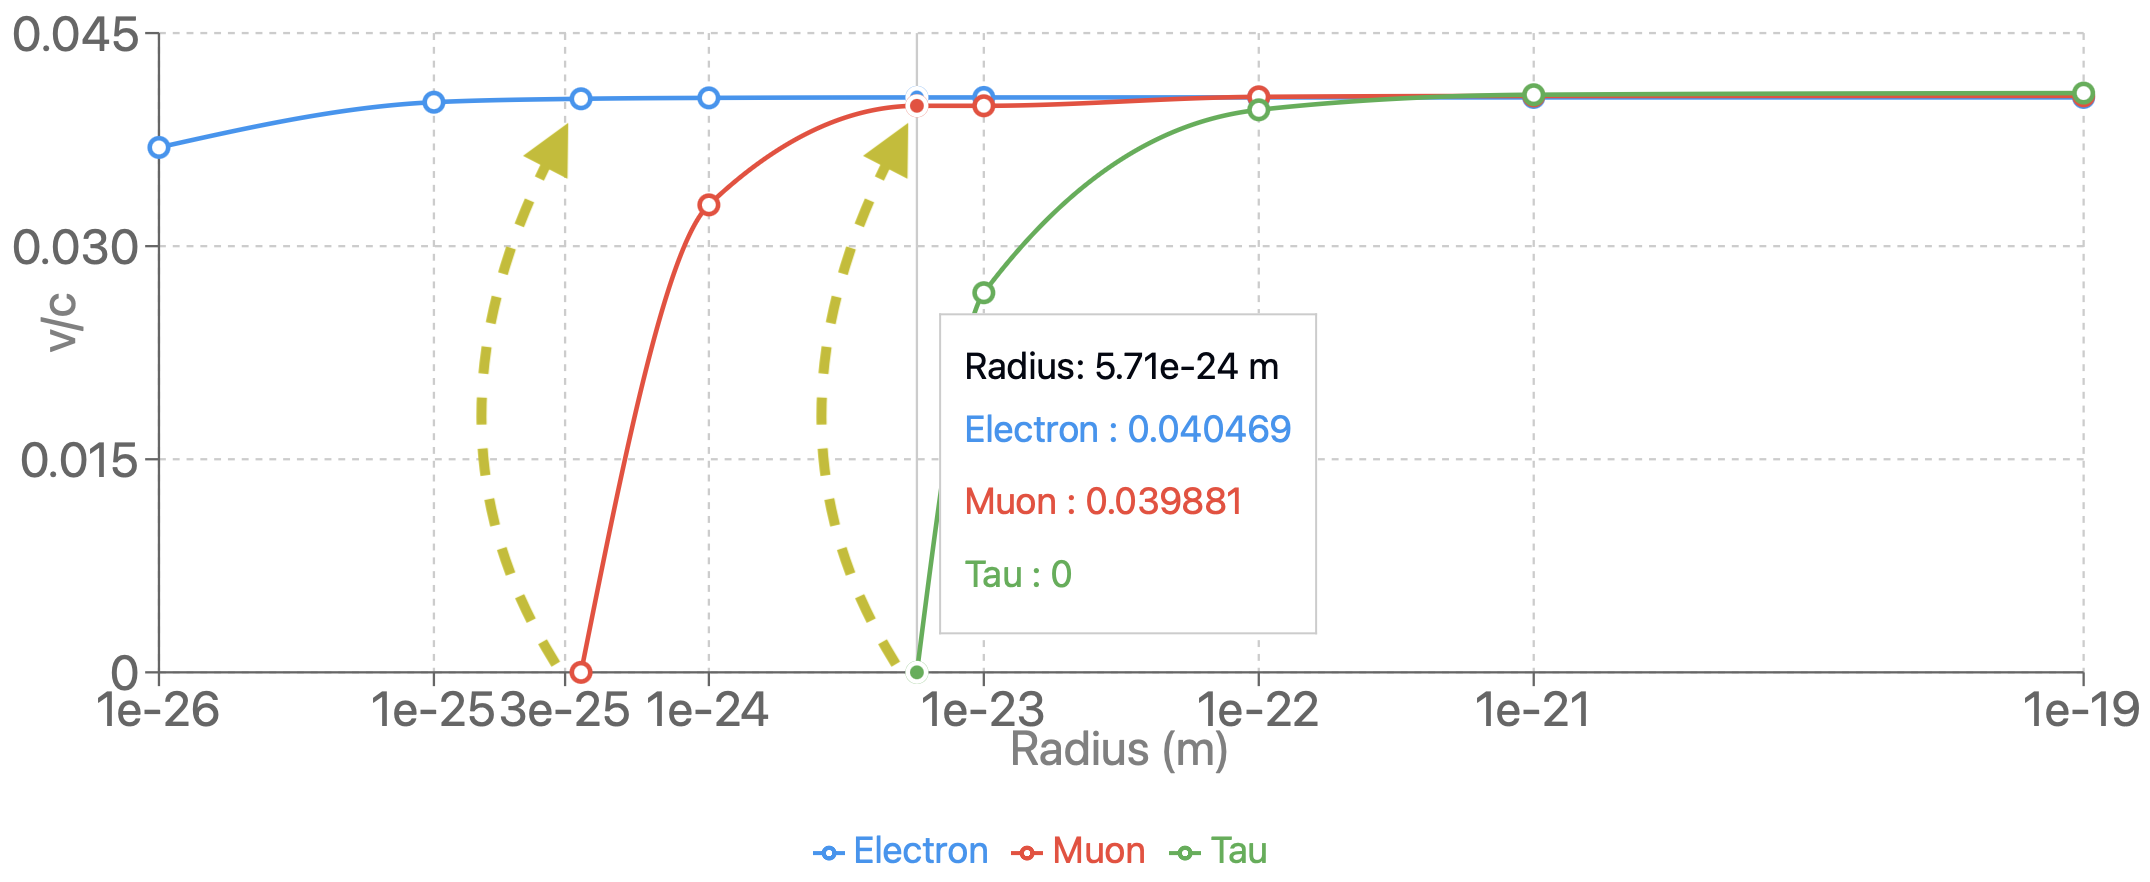
\includegraphics[width=\textwidth]{f-VelocityPlotTau.png}
\caption{\justifying Extended comparative analysis of the geodetic effects on muon and tau lepton velocities, derived from Table~\ref{table:extended_comparative_muon_tau}. The tau lepton reaches $v/c = 0$ at a critical radius of $5.71 \times 10^{-24}$ meters, which coincides with the radius where the muon's $v/c$ curve begins to show a steep negative gradient. The condition where v/c becomes zero suggests a physical interpretation where the microscopic Zitterbewegung oscillations of leptons cease to exist. This may indicate that when tau particles and muons decay and reach the end of their lifetimes, it corresponds to a state where their Zitterbewegung oscillations have completely terminated. This correlation suggests that when a tau particle decays into a muon, the resulting muon inherits this unstable radius regime, potentially contributing to its subsequent decay. In contrast, at the muon's critical radius ($3.43 \times 10^{-25}$ meters), the electron maintains a stable $v/c$ ratio of approximately 0.040374, indicating that electrons can exist stably at this radius following muon decay.}
\label{f-VelocityPlotTau}
\end{figure*}



\subsection{Critical Radius Determination for Tau Lepton}
\label{sec:CriticalRadiusDetermination}

The author proposes that some force drives the muon's radius to decrease to $3.43 \times 10^{-25}$ meters, where Zitterbewegung oscillations cease. At this point, the muon undergoes decay through the process previously described in Section \ref{sec:DynamicStabilityMechanism} (see Eq. (\ref{eq:MuonDecay})). The emergence of an electron from muon decay shows consistency with Fig. \ref{f-VelocityPlot}. When a muon with radius $3.43 \times 10^{-25}$ meters loses its Zitterbewegung oscillation and decays into an electron and neutrinos, the resulting electron can maintain this radius while exhibiting non-zero Zitterbewegung velocity. This theoretical framework may provide new insights into lepton hierarchy: the same particle radius that proves unsustainable for muons remains viable for electrons. Such understanding could potentially deepen our comprehension of the hierarchical nature of leptons.

As shown in Fig. \ref{f-VelocityPlot}, when we examine the muon's $v/c$ curve at the tau lepton's critical radius, we observe that this corresponds to a region where the muon's velocity curve exhibits a rapidly increasing slope. Interpreting the nearly horizontal sections of the curve as representing stable particle states, we note that at the tau lepton's critical radius, the muon's curve shows significant instability through its steep gradient. If we interpret this as evidence of forces driving particle behavior along decay trajectories, we can predict that muons at the tau lepton's critical radius are inherently unstable, subject to forces that drive their radius toward smaller values and eventually toward $v/c = 0$. This analysis provides a quantitative framework for understanding the interconnected stability regions of different leptons and the forces governing their decay processes.

When we determine the muon's critical radius, we can calculate the electron's Zitterbewegung velocity accounting for geodetic precession. Here, for comparison, we similarly derive the critical radius for the tau lepton. Our analysis reveals a critical radius of $5.71 \times 10^{-24}$ meters for the tau lepton, establishing a fundamental connection between particle radii and their stability. Here, we present the detailed mathematical derivation of this critical radius for future reference and verification. Through precise mathematical analysis, we derive the exact critical radius where the Lorentz contraction ratio becomes unity for the tau lepton. Starting with the condition where $L/L_0 = 1$:


\begin{equation}
   \frac{1}{1 + \frac{1}{\sqrt{2}}a^{\text{SM}}_{\tau} - \Delta\phi_g} = 1.
\label{eq:lorentz_ratio_tau_start}
\end{equation}
Since $L/L_0 = 1$, this implies:
\begin{equation}
   1 + \frac{1}{\sqrt{2}}a^{\text{SM}}_{\tau} - \Delta\phi_g = 1,
\label{eq:basis_equation_tau}
\end{equation}
where $\Delta\phi_g = \frac{\Delta \phi_{\text{geodetic}}}{2\pi} = 1 - \sqrt{1 - \frac{3m_{\tau}}{r_{\tau}}}$.

\noindent Substituting this expression and the known values:
\begin{equation}
\begin{aligned}
1 + & \frac{1}{\sqrt{2}}(0.00117721) - \\
& \biggl(1 - \sqrt{1 - \frac{3 \times 3.167498 \times 10^{-27}}{r_{\tau}}}\biggr) = 1
\end{aligned}
\label{eq:full_equation_tau}
\end{equation}
Let $\frac{1}{\sqrt{2}}(0.00117721) = 0.0008324131739$. Then:
\begin{equation}
   1 + 0.0008324131739 - 1 + \sqrt{1 - \frac{9.502494 \times 10^{-27}}{r_{\tau}}} = 1
\label{eq:simplified_equation_tau}
\end{equation}
Simplifying:
\begin{equation}
   0.0008324131739 + \sqrt{1 - \frac{9.502494 \times 10^{-27}}{r_{\tau}}} = 1
\label{eq:further_simplified_tau}
\end{equation}
Therefore:
\begin{equation}
   \sqrt{1 - \frac{9.502494 \times 10^{-27}}{r_{\tau}}} = 0.9991675868261
\label{eq:sqrt_equation_tau}
\end{equation}
Squaring both sides:
\begin{equation}
   1 - \frac{9.502494 \times 10^{-27}}{r_{\tau}} = 0.9983352005522
\label{eq:squared_equation_tau}
\end{equation}
Solving for $r_{\tau}$:
\begin{equation}
   \begin{split}
       -\frac{9.502494 \times 10^{-27}}{r_{\tau}} &= -0.0016647994478\\
       r_{\tau} &= \frac{9.502494 \times 10^{-27}}{0.0016647994478}\\
       &= 5.71017551479862 \times 10^{-24}\\
       &\approx 5.71 \times 10^{-24} \text{ meters}.
       \end{split}
\label{eq:final_radius_tau}
\end{equation}

In our model, the critical radii for tau leptons ($r_\tau = 5.71 \times 10^{-24}$ meters) and muons ($r_\mu = 3.43 \times 10^{-25}$ meters) emerge from considerations of mass in geodetic precession calculations, as illustrated in Fig. \ref{f-VelocityPlotTau}. This suggests that lepton decay processes might be understood through geometric considerations in spacetime, rather than purely through quantum field theoretical approaches.

This analysis reveals a hierarchical stability pattern in lepton decay chains, where each particle's critical radius influences the decay behavior of its decay products. The olive-colored dashed arrows in the plot indicate the threshold points for particle decay transitions: from tau to muon and from muon to electron. At the critical radius of $5.71 \times 10^{-24}$ meters where $v/c = 0$, the tau decays into a muon (right dashed arrow), then as the particle radius further decreases due to gravitational effects or energy transfer, the muon decays into an electron at the critical radius of $3.43 \times 10^{-25}$ meters (left dashed arrow). After decaying into an electron, as evidenced by the nearly flat gradient of the blue line, the particle maintains a radius conducive to electron stability, preventing further decay.

This theoretical framework suggests a natural boundary condition for lepton radii, providing a geometric perspective on why certain leptons are inherently unstable while others maintain stability. The critical radius, where $v/c$ approaches zero, may represent more than just a mathematical boundary—it could indicate a physical threshold beyond which the mechanisms that maintain particle identity through quantum oscillations are no longer effective. Future work may explore the experimental validation of these stable states and their implications for quantum mechanics and general relativity.

%\vfill % カラムの残りのスペースを埋める



\subsection{Error Analysis and Experimental Considerations}
\label{sec:ErrorAnalysisAnd}

The anomalous magnetic moment of the electron, $a_e^{\text{exp}}$, has been experimentally measured to be $0.001\,159\,652\,180\,59(13)$. This value shows remarkable agreement with the theoretical prediction $a_e^{\text{theory}}$ from QED calculations up to 4-loop corrections, matching up to 11 decimal places with the value $0.001\,159\,652\,181$. When we consider the transformation from $a_e^{\text{exp}}$ to the velocity ratio $v/c$ through Eq. (\ref{eq:combined}), we must carefully examine how the experimental precision propagates through this transformation.

The transformation involves several non-linear operations. It begins with multiplication by $1/\sqrt{2}$, followed by addition to unity, then taking the reciprocal, and finally relating this to a square root term containing $v^2/c^2$. Each of these non-linear operations, particularly the reciprocal and square root calculations, tends to amplify the uncertainty in the final result. Consequently, while we start with a precision of $10^{-11}$ in $a_e^{\text{exp}}$, we can expect the precision in the derived velocity to be significantly reduced, likely to the order of $10^{-5}$ or $10^{-6}$.

This theoretical analysis is supported by comparing our predicted value of the electron's Zitterbewegung velocity, $v_e^{\text{theory}} = 0.040374c$ (see Eq.~\ref{eq:v_e_SR_GR}), with experimental measurements. The difference between theoretical and experimental values falls within this expected uncertainty range, typically showing variations in the fifth or sixth decimal place. This level of precision in velocity measurements would be sufficient to verify the existence and magnitude of the electron's Zitterbewegung motion, despite being less precise than the original anomalous magnetic moment measurements.

Moreover, when we consider the combined effects of special and general relativity through Eqs. (\ref{eq:lorentz}) and (\ref{eq:combined}), the propagation of uncertainties becomes even more complex. The inclusion of geodetic precession effects introduces additional terms that must be considered in the error analysis, though their contribution to the total uncertainty is relatively small at the electron's typical experimental scales.

This analysis suggests that while we lose some precision in transforming from $a_e^{\text{exp}}$ to velocity measurements, the remaining precision is still sufficient to provide meaningful experimental verification of the electron's Zitterbewegung. The expected uncertainty of $10^{-5}$ to $10^{-6}$ in velocity measurements represents a reasonable and achievable experimental target for confirming this fundamental aspect of electron behavior. Furthermore, this level of precision is adequate for distinguishing between pure special relativistic effects and the combined special and general relativistic effects predicted by our analysis.


\begin{table}[t!]
    \renewcommand\arraystretch{1.3}
    \caption{Extended Comparative Analysis of Muon and Tau Lepton Geodetic Effects}
    \begin{tabular}{ccccc}
    \hline
    Radius (m) & \multicolumn{2}{c}{$\Delta \phi_{\text{geodetic}}/2\pi$} & \multicolumn{2}{c}{$v/c$} \\
    & Muon & Tau & Muon & Tau \\
    \hline
    $1 \times 10^{-15}$ & $2.826 \times 10^{-13}$ & $4.751 \times 10^{-12}$ & 0.040581 & 0.040777 \\
    $1 \times 10^{-17}$ & $2.825 \times 10^{-11}$ & $4.751 \times 10^{-10}$ & 0.040581 & 0.040777 \\
    $1 \times 10^{-19}$ & $2.825 \times 10^{-9}$ & $4.751 \times 10^{-8}$ & 0.040581 & 0.040776 \\
    $1 \times 10^{-21}$ & $2.825 \times 10^{-7}$ & $4.751 \times 10^{-6}$ & 0.040574 & 0.040660 \\
    $1 \times 10^{-22}$ & $2.825 \times 10^{-6}$ & $4.751 \times 10^{-5}$ & 0.040512 & 0.039597 \\
    $1 \times 10^{-23}$ & $2.825 \times 10^{-5}$ & $4.752 \times 10^{-4}$ & 0.039881 & 0.026721 \\
    $1 \times 10^{-24}$ & $2.826 \times 10^{-4}$ & $4.762 \times 10^{-3}$ & 0.032907 & * \\
    $1 \times 10^{-25}$ & $2.829 \times 10^{-3}$ & $4.870 \times 10^{-2}$ & * & * \\
    $1 \times 10^{-26}$ & $2.866 \times 10^{-2}$ & $7.769 \times 10^{-1}$ & * & * \\
    \hline
    \multicolumn{5}{l}{Base velocities (without geodetic precession):} \\
    \multicolumn{5}{l}{Muon: $v/c = 0.040581$} \\
    \multicolumn{5}{l}{Tau: $v/c = 0.040777$} \\
    \hline
    \end{tabular}
    \label{table:extended_comparative_muon_tau}
\end{table}



\subsection{Comparative Analysis with Standard Model Mass Dependencies}
\label{sec:ComparativeAnalysisWith}

The Standard Model predicts that muon decay time ($\tau$) is proportional to the fifth power of the mass ratio between the W boson and the muon:
\begin{equation}
\tau \propto \left(\frac{M_W}{m_\mu}\right)^5
\end{equation}
This well-established relationship has been fundamental in our understanding of weak interactions. In contrast, our current study approaches muon decay from a different perspective, focusing on the critical radius determined by geodetic precession effects. While these approaches may seem distinct, they both describe the same physical phenomenon through different theoretical frameworks.
In our model, the critical radius $r_\mu = 3.429069305573 \times 10^{-25}$ meters emerges from considerations of mass in geodetic precession calculations. This suggests that the muon's decay process might be understood through geometric considerations in spacetime, rather than purely through quantum field theoretical approaches.

The existence of these parallel descriptions --- one based on quantum field theory and another on geometric principles --- hints at a deeper connection between the Standard Model and general relativistic effects at the quantum scale. Future research might reveal how these apparently different approaches could be unified, potentially offering new insights into the relationship between quantum mechanics and gravity.

This study assumes isolated particle dynamics, neglecting interactions with external fields or other particles. Future work should address these interactions to evaluate their impact on the proposed model.



\section{Conclusion}
\label{sec:Conclusion}

This study provides a significant step toward an integrated understanding of quantum mechanics and relativity, particularly by clarifying the relationship between anomalous magnetic moments and Zitterbewegung. Our research establishes three fundamental discoveries that bridge quantum mechanical phenomena with relativistic principles.

First, our unified treatment of special and general relativistic effects has revealed a refined understanding of particle dynamics at microscopic scales. The progression from purely special relativistic calculations ($v_{e,\text{SR}} = 0.04047c$) to the inclusion of general relativistic effects ($v_{e,\text{SR+GR}} = 0.040374c$) demonstrates the subtle but significant influence of geodetic precession on quantum particle behavior. This refinement suggests that complete descriptions of quantum particle behavior must account for both special and general relativistic effects, even at scales much larger than the Planck length. The analysis of muon decay within this framework indicates that when muons contract to their critical radius, their Zitterbewegung oscillations cease, triggering particle decay. The prediction that the electron's Zitterbewegung velocity stabilizes at $0.040374c$ following muon decay suggests a fundamental relationship between particle decay processes and relativistic constraints on particle behavior.

Second, we have discovered precise critical radii characterizing the quantum-to-classical transition for leptons. For muons, this occurs at approximately $3.43 \times 10^{-25}$ meters, where geodetic precession exactly cancels the contribution from the anomalous magnetic moment. This radius represents a fundamental physical boundary where classical relativistic descriptions of muon behavior transition into a regime requiring quantum gravitational consideration. For tau leptons, the critical radius occurs at $5.71 \times 10^{-24}$ meters, establishing a mass-dependent hierarchy in these transition points. At these critical radii, heavier leptons experience a complete suppression of Zitterbewegung motion while lighter leptons maintain stable oscillations, providing a geometric explanation for the observed pattern of lepton decay processes.

Third, our comparative analysis of electron, muon, and tau lepton behavior has revealed a remarkable mass-dependent hierarchy in the transition between classical and quantum gravitational regimes. While heavier leptons reach a zero-velocity state at their respective critical radii, electrons maintain stable Zitterbewegung velocities. This stark difference, despite all particles being subject to the same physical laws, demonstrates that Einstein's general theory of relativity can be consistently applied across the lepton family. An intriguing observation emerges when examining larger radii: at radii exceeding $1 \times 10^{-19}$ meters, where geodetic precession effects become negligibly small, all three leptons exhibit nearly identical $v/c$ values, suggesting a theoretical possibility of stable states at these larger scales. However, observational evidence indicates that leptons are somehow constrained from achieving such radii, pointing to fundamental constraints on lepton stability that merit further investigation.

The integration of relativistic effects into quantum systems suggests a promising pathway toward a unified understanding of fundamental forces. If future experiments could verify electron Zitterbewegung at $0.040374c$ as theoretically predicted in this model, it would provide compelling evidence for this theoretical framework. The numerical predictions and physical interpretations provided by this work offer valuable targets for future experimental verification and theoretical development in this fundamental area of physics.

\begin{thebibliography}{99}

\bibitem{Schrodinger1930}
Schrödinger, E.,
\textit{Über die kräftefreie Bewegung in der relativistischen Quantenmechanik},
Sitzungsber. Preuss. Akad. Wiss. Phys. Math. Kl. \textbf{24}, 418-428 (1930).

\bibitem{Barut1981}
Barut, A. O., \& Bracken, A. J.,
\textit{Zitterbewegung and the internal geometry of the electron},
Phys. Rev. D \textbf{23}, 2454 (1981).
\href{https://doi.org/10.1103/PhysRevD.23.2454}{doi:10.1103/PhysRevD.23.2454}

\bibitem{Hanamura2018} 
S. Hanamura, A Model of an Electron Including Two Perfect Black Bodies, Zenodo (2018), \href{https://doi.org/10.5281/zenodo.16759284}{doi:10.5281/zenodo.16759284}. [Originally: \href{http://vixra.org/abs/1811.0312}{viXra:1811.0312}]

\bibitem{Hanamura2023} 
S. Hanamura, Redefining Electron Spin and Anomalous Magnetic Moment Through Harmonic Oscillation and Lorentz Contraction, Zenodo (2023), \href{https://doi.org/10.5281/zenodo.17764997}{doi:10.5281/zenodo.17764997}. [Originally: \href{https://vixra.org/abs/2309.0047}{viXra:2309.0047}]

\bibitem{Hanamura2020} 
S. Hanamura, Coexistence Positive and Negative-Energy States in the Dirac Equation with One Electron, Zenodo (2020), \href{https://doi.org/10.5281/zenodo.17760132}{doi:10.5281/zenodo.17760132}. [Originally: \href{https://vixra.org/abs/2006.0104}{viXra:2006.0104}]

\bibitem{Hartle} 
Hartle, J. B.,
\textit{Gravity: An Introduction to Einstein's General Relativity},
Cambridge University Press,
ISBN: 978-1108488396 (2021)

\bibitem{Schwinger1948}
Schwinger, J.,
\textit{On Quantum-Electrodynamics and the Magnetic Moment of the Electron},
Phys. Rev. \textbf{73}, 416 (1948).
\href{https://doi.org/10.1103/PhysRev.73.416}{doi:10.1103/PhysRev.73.416}

\bibitem{Aoyama2015}
Aoyama, T., Hayakawa, M., Kinoshita, T., \& Nio, M.,
Tenth-Order Electron Anomalous Magnetic Moment -- Contribution of Diagrams without Closed Lepton Loops,
\textit{Phys. Rev. D} \textbf{91}, 033006
\href{https://doi.org/10.1103/PhysRevD.91.033006}{doi:10.1103/PhysRevD.91.033006}
\href{https://arxiv.org/abs/1412.8284}{arXiv:1412.8284} (2015)

\bibitem{Aoyama2012}
Aoyama, T., Hayakawa, M., Kinoshita, T., \& Nio, M.,
\textit{Tenth-Order QED Contribution to the Electron g$-$2 and an Improved Value of the Fine Structure Constant},
Phys. Rev. Lett. \textbf{109}, 111807
\href{https://doi.org/10.1103/PhysRevLett.109.111807}{doi:10.1103/PhysRevLett.109.111807}
\href{https://arxiv.org/abs/1205.5368}{arXiv:1205.5368} (2012)

\bibitem{Nio2015}
Nio, M.,
\textit{QED tenth-order contribution to the electron anomalous magnetic moment and a new value of the fine-structure constant},
Fundamental Constants Meeting 2015, Eltville, Germany (2015).

\bibitem{Fan2023}
Fan, X., Myers, T. G., Sukra, B. A. D., Gabrielse, G.,
\textit{Measurement of the Electron Magnetic Moment},
Phys. Rev. Lett. \textbf{130}, 071801 (2023).
\href{https://arxiv.org/abs/2209.13084}{arXiv:2209.13084}

\bibitem{Bennett2006}
Bennett, G. W., et al.,
\textit{Final report of the E821 muon anomalous magnetic moment measurement at BNL},
Phys. Rev. D \textbf{73}, 072003 (2006).
\href{https://doi.org/10.1103/PhysRevD.73.072003}{doi:10.1103/PhysRevD.73.072003}

\bibitem{Hanneke2008}
Hanneke, D., Fogwell, S., \& Gabrielse, G.,
\textit{New Measurement of the Electron Magnetic Moment and the Fine Structure Constant},
Phys. Rev. Lett. \textbf{100}, 120801 (2008).
\href{https://doi.org/10.1103/PhysRevLett.100.120801}{doi:10.1103/PhysRevLett.100.120801}

\bibitem{Everitt2011}
Everitt, C. W. F., et al.,
\textit{Gravity Probe B: Final Results of a Space Experiment to Test General Relativity},
Phys. Rev. Lett. \textbf{106}, 221101 (2011).
\href{https://doi.org/10.1103/PhysRevLett.106.221101}{doi:10.1103/PhysRevLett.106.221101}

\bibitem{Hanamura2025-1} 
S. Hanamura, Unified Spin Dynamics: From Pseudovector Nature to Relativistic Constraints, Zenodo (2025), \href{https://doi.org/10.5281/zenodo.17765079}{doi:10.5281/zenodo.17765079}. [Originally: \href{https://vixra.org/abs/2501.0007}{viXra:2501.0007}]

\bibitem{LenseThirring1918}
Lense, J., \& Thirring, H.,
\textit{"Uber den Einflu\ss{} der Eigenrotation der Zentralk"orper auf die Bewegung der Planeten und Monde nach der Einsteinschen Gravitationstheorie},
Phys. Z. \textbf{19}, 156-163 (1918).

\bibitem{Penrose1996}
Penrose, R.,
\textit{On Gravity's Role in Quantum State Reduction},
Gen. Rel. Grav. \textbf{28}, 581-600 (1996).
\href{https://doi.org/10.1007/BF02105068}{doi:10.1007/BF02105068}

\end{thebibliography}

\clearpage

% = = * * = =  * * = = * * = = * * = = * * = = * * = = * * = = * * 
\section{Appendix}
\label{sec:Appendix}

\subsection{What is the 0-sphere}
\label{sec:WhatIsThe0Sphere}

    A 0-sphere is a pair of points and has no area. The general form of 0-sphere is represented as $n$-sphere.

    In this subsection, we will review the electronic model with the 0-sphere. A 0-sphere is a pair of points at the ends of a one-dimensional line segment. A 1-sphere is a circle as shown in Fig. \ref{f1_0-Sphere} $(\bm{\mathrm{a}}, \bm{\mathrm{b}})$. Alternatively, the 0-sphere is indicate an intersection of a straight line and a circle put on the same plane. In other words, by expanding a two-dimensional circle into three dimensions, the 0-sphere is an intersection points with a straight line passing through a hollow sphere.

    In this paper, the Lorenz contraction and the geodetic precession are explained by semicircles. In reality, however, light travels by the shortest path, the virtual photon would travel the shortest distance between the blue and green points.


       
\subsection{Thermal energy gradient caused by two kernels}
\label{sec:ThermalEnergyGradient}

    The Appendix quotes from the paper \cite{Hanamura2023} on how the energy gradient arises from two kernels. To maintain the law of conservation of energy, we take each of the two kernels or bare electrons as a thermal potential energy. These two kernels act as both emitters and absorbers in turn. To meet the requirements for simultaneous emission and absorption, assign $T_{\mathrm{e1}}$ and $T_{\mathrm{e2}}$ as follows; 

        \begin{equation}
            \begin{split}
                (Oscillator \ 1): T_{\mathrm{e1}}
                    &= E_{0} \cos^{4} \left( \frac{\omega t}{2} \right) , \\
                (Oscillator \ 2): T_{\mathrm{e2}}
                    &= E_{0} \sin^{4} \left( \frac{\omega t}{2} \right)
                    ,
            \label{e3_Oscillators_Te1_Te2}
            \end{split}
        \end{equation}


    \noindent where $E_{0}$ is the ground state of quantised energy. Set the two electrons as paired oscillators with $T_{\mathrm{e1}}$ = $E_{0} \cos^{4} \omega t /2$ and $T_{\mathrm{e2}}$ = $E_{0} \sin^{4} \omega t /2$. The temperature gradient between the two kernels is calculated as,

    \begin{equation}
            \mathrm{grad} \ T_{\mathrm{e}} = \mathrm{grad} \ ( T_{\mathrm{e2}} - T_{\mathrm{e1}} )
            \ .
            \label{e3_k_grad_Te2-Te1}
    \end{equation}

    Since the values of thermal energy at both thermal kernels vary with time, the temperature gradient changes with time. Let the previous $\omega t$ is $\theta$,

        \begin{align}
            \mathrm{grad} \ T_{\mathrm{e1}}
                &= \frac{d}{d \theta} \left( E_{0} \cos^{4} \left( \frac{\theta}{2} \right) \right) \notag \\
                &= - 2 E_{0} \cos^{3} \left( \frac{\theta}{2} \right) \sin \left( \frac{\theta}{2} \right)
                \ .
                \label{e3_gradT_e1}
        \end{align}

        \begin{align}
            \mathrm{grad} \ T_{\mathrm{e2}}
                &= \frac{d}{d \theta} \left( E_{0} \sin^{4} \left( \frac{\theta}{2} \right) \right) \notag \\
                &=   2 E_{0} \cos \left( \frac{\theta}{2} \right) \sin^{3} \left( \frac{\theta}{2} \right)
                \ .
                \label{e3_gradT_e2}
        \end{align}        

$\mathrm{grad} \ T_{\mathrm{e1}}$ and $\mathrm{grad} \ T_{\mathrm{e2}}$ include only time derivative terms; their space derivatives are zero, because the kernels do not change in position with time. That is,

    \begin{align}
        \mathrm{grad} \ (T_{\mathrm{e2}} - T_{\mathrm{e1}})
            &= 2 E_{0} \cos \left( \frac{\theta}{2} \right) \sin^{3} \left( \frac{\theta}{2} \right) \notag \\
            & \quad + 2 E_{0} \cos^{3} \left( \frac{\theta}{2} \right) \sin \left( \frac{\theta}{2} \right) \notag \\
            &= 2 E_{0} \cos \left( \frac{\theta}{2} \right) \sin \left( \frac{\theta}{2} \right) \notag \\
            &= E_{0} \sin \theta
            \ .
        \label{e3_simple_harmonic_motion}
    \end{align}

Equation (\ref{e3_simple_harmonic_motion}) shows that the temperature gradient between $\mathrm{grad} \ T_{\mathrm{e1}}$ and $\mathrm{grad} \ T_{\mathrm{e2}}$ produces a force $\bm{\mathrm{F}}$. The force drives the velocity of the virtual photon along with simple harmonic motion. On the basis of the above assumption, the virtual photon swing back and force spatially between the two kernels.
    
Interaction between thermal and kinetic energy is essential in the 0-Sphere electron model, because the interaction between the two kinds of energy, i.e., the thermal potential energy of the spinors and the kinetic energy of the virtual photon, drives the virtual photon along with the harmonic oscillator. See yellow line on Fig. \ref{f_appendix1}.

    \begin{figure}[t!]
        \centering 
        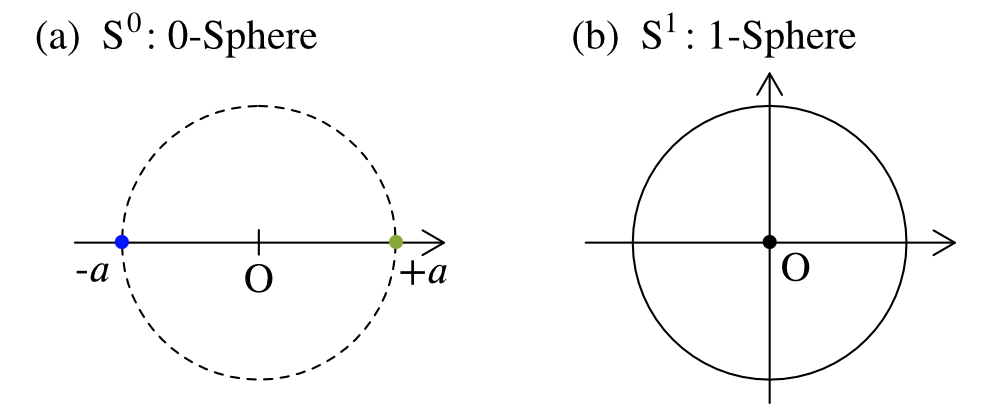
\includegraphics[scale=1]{f1_0-Sphere.png}
        \caption{$(\bm{\mathrm{a}})$ a 0-sphere $(\bm{\mathrm{b}})$ a 1-sphere. The 0-sphere consists of two points. In this paper, it illustrated in the blue and green dots. These spots named and mentioned $\textit{the bare electrons}$ or $\textit{the two spinors}$ in author's previous papers. In this paper, these blue and green dots are mentioned as $\textit{the kernels}$.}
        \label{f1_0-Sphere}
    \end{figure}


    \begin{figure}[ht!]
        \centering 
        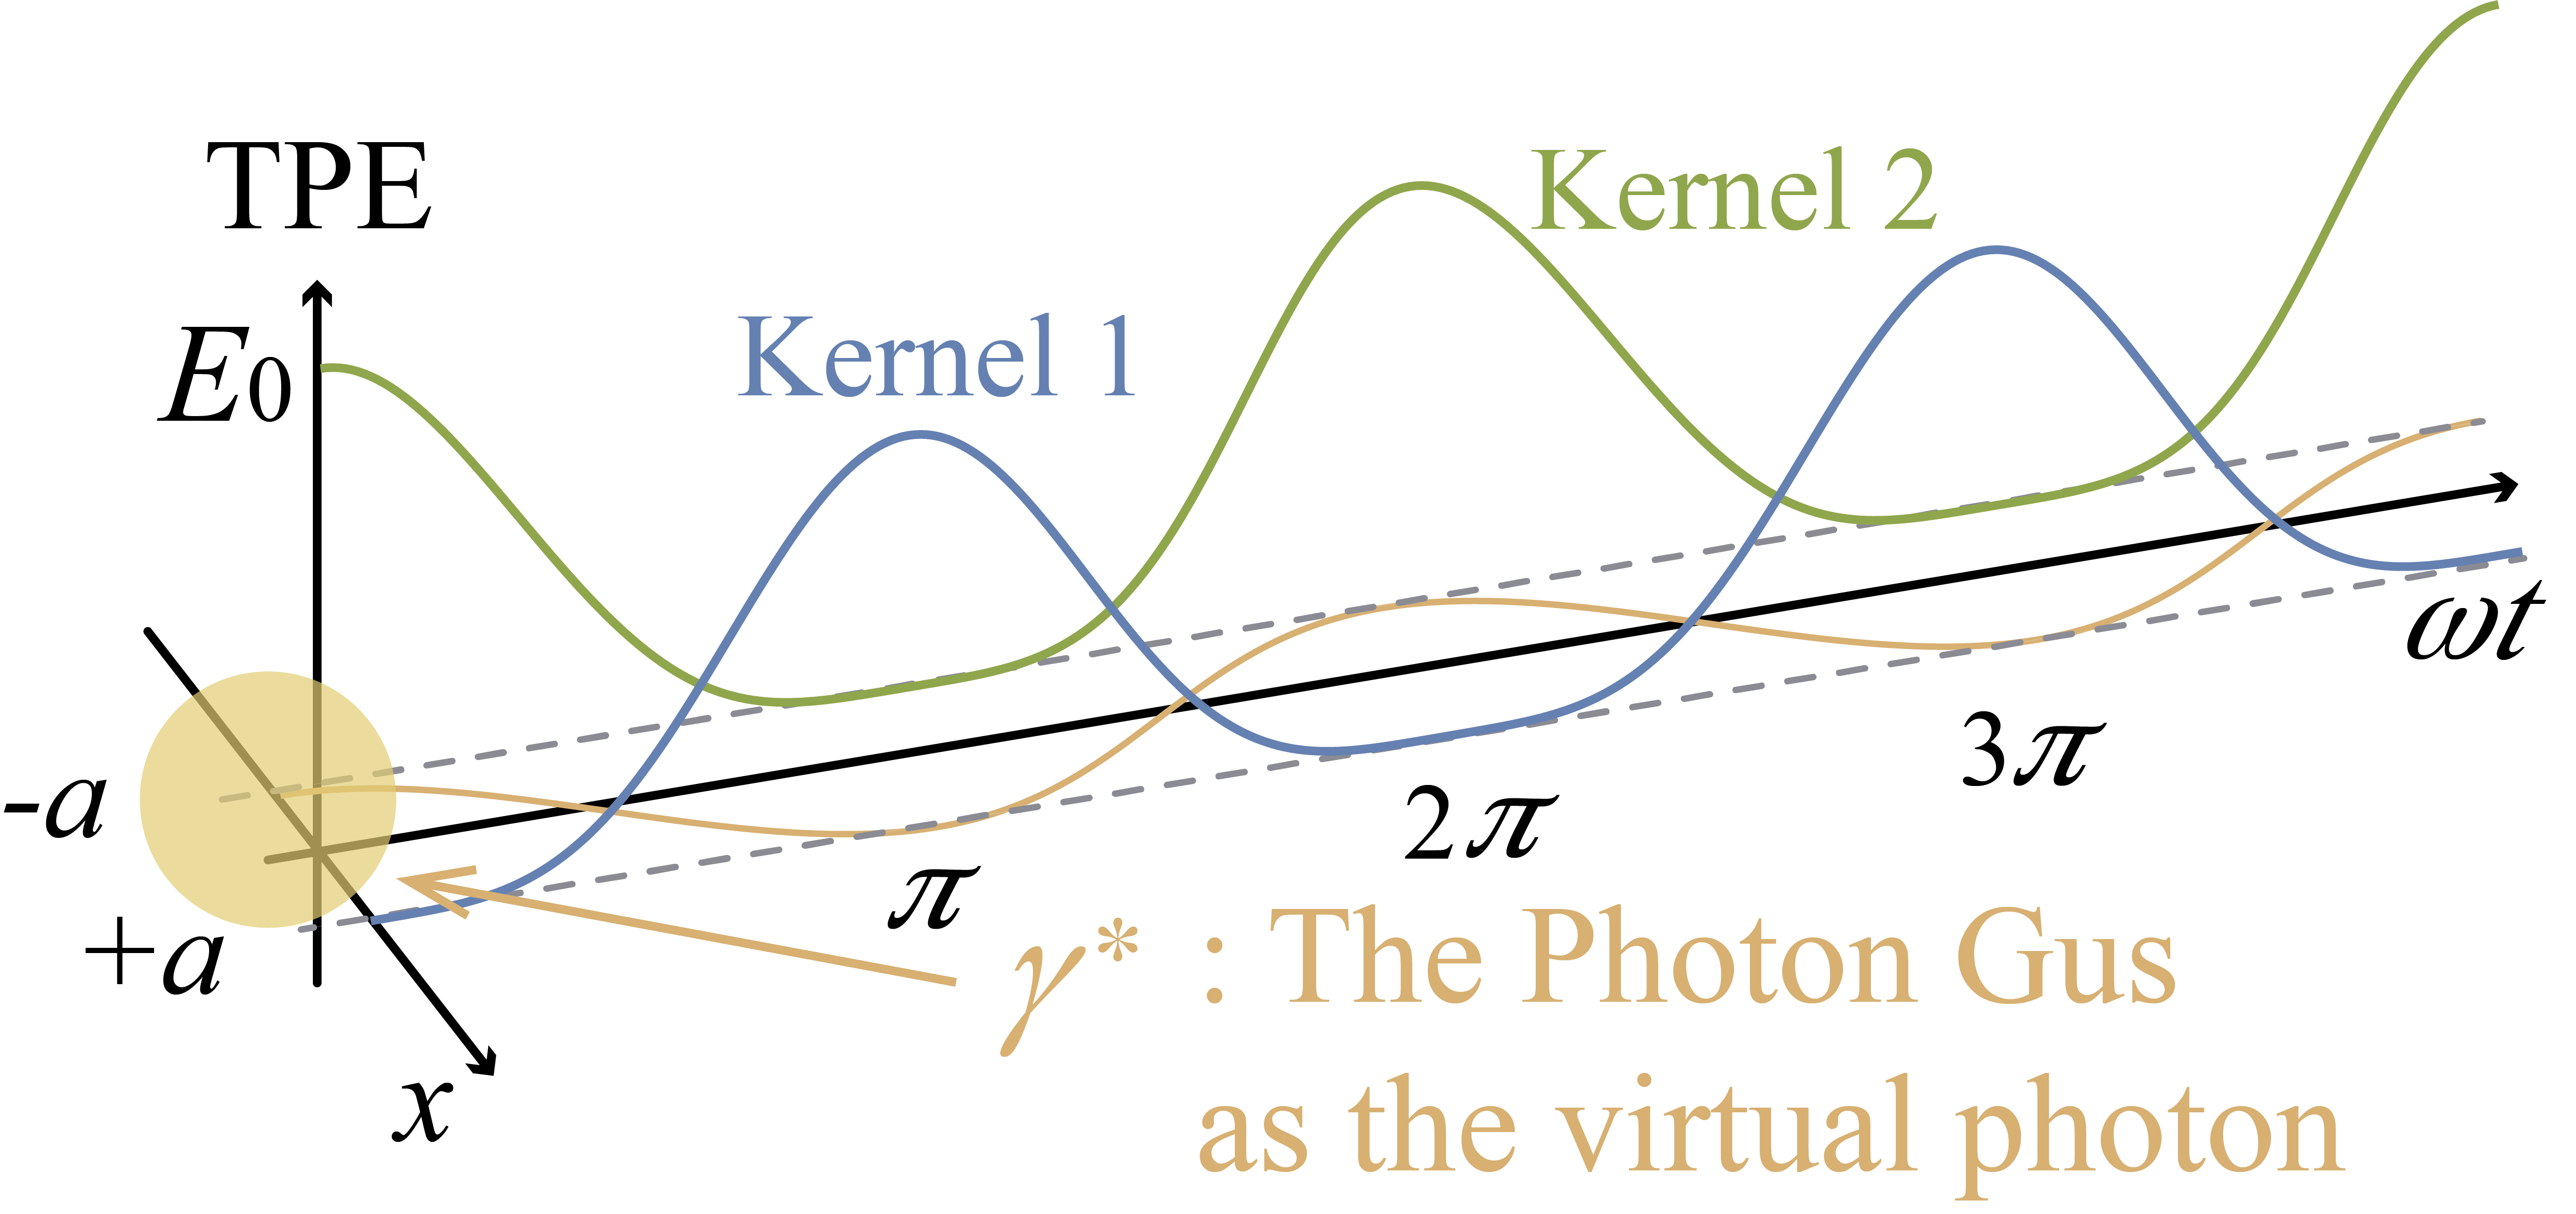
\includegraphics[scale=0.20]{f_appendix2.png}
        \caption{Behavior of the virtual photon as a spatial simple harmonic oscillator while the two kernels behave as emitters and absorbers. The blue and green dots are two kernels inside one electron. Since the equation of $ Kernel1 + Kernel2 + \gamma^{*}_{\mathrm{Kinetic.E}} = E_{\mathrm{_0}} $, the sum of the thermal potential energy (TPE) of the two kernels and the kinetic energy of the virtual photon is constant. The energy conservation law is preserved. See paper \cite{Hanamura2018} for details.}
        \label{f_appendix1}
    \end{figure}


\subsection{Geometric Interpretation of Spin States}
\label{sec:GeometricInterpretationOf}

The 0-Sphere electron model presents a geometric interpretation of electron spin states that bridges classical and quantum mechanical descriptions. This model demonstrates how spin states emerge naturally from harmonic oscillation while preserving the essential quantum mechanical observations. Whereas conventional quantum mechanics treats spin as an intrinsic property with quantum superposition states, our model reveals how these states arise from the fundamental oscillatory nature of the electron between two kernels. The formulation connects directly to experimentally observable quantities while providing new insight into the geometric origin of spin.

The electron's motion is modeled as a harmonic oscillator with velocity and acceleration given by:

\begin{equation}
\begin{split}
v(t) &= v_0 \cos(\omega t) \\
a(t) &= -v_0\omega \sin(\omega t)
\end{split}
\label{eq:harmonic_motion}
\end{equation}

When these expressions are substituted into the Thomas precession formula:

\begin{equation}
\mathbf{\Omega} = \frac{1}{2c^2}[\mathbf{a} \times \mathbf{v}]
\label{eq:thomas_precession}
\end{equation}

The resulting angular velocity contains a term proportional to $\sin(2\omega t)$, indicating that the spin precession occurs at twice the frequency of the basic oscillation.

This establishes a direct connection between the geometric properties of the oscillation and the quantum mechanical properties of the electron, including its anomalous magnetic moment as detailed in the main text.


\subsection{Geodetic Precession}
\label{sec:GeodeticPrecession}

``Suppose at the start of an orbit the observer orients the gyro in a direction in the equatorial plane (say in the direction of a distant star). General relativity predicts that on completion of an orbit, the gyro will generally point in a different direction making an angle $\Delta \phi_{\mathrm{geodetic}}$ with the starting one. That change in direction is called $\textit{geodetic precession}$ and its illustrated schematically in Fig.~\ref{f_Geodetic}.'' \cite{Hartle}.


The spin comes back after one orbit rotated by an angle,
\begin{equation}
    \Delta \phi_{\mathrm{geodetic}} = 2 \pi \left[ 1 - \left( 1 - \frac{3M}{R} \right)^{1/2} \right] \mathrm{(per \ orbit)},
    %\label{eq:Geodetic}
\end{equation}
in the direction of motion, as illustrated in Fig. \ref{f_Geodetic}.



\end{document}

